\documentclass[12pt,twoside,openany]{book}

\input macros

\begin{document}

\frontmatter
\cfoot[{\eng{\thepage}}]{{\eng{\thepage}}}
\makeatletter

\def\@makechapterhead#1{%
  \vspace*{10\p@}%
  {\parindent \z@ \centering \normalfont
    \ifnum \c@secnumdepth >\m@ne
      %~ \if@mainmatter
        %~ \huge\bfseries \@chapapp\space \thechapter
        %~ \par\nobreak
        %~ \vskip 20\p@
      %~ \fi
    \fi
    \interlinepenalty\@M
    \kannadafont\Huge \bfseries #1\par\nobreak
    \vskip 15\p@
}}

\def\@part[#1]#2{%
    \ifnum \c@secnumdepth >-2\relax
      \refstepcounter{part}%
      \addcontentsline{toc}{part}{\eng{\thepart}\hspace{1em}#1}%
    \else
      \addcontentsline{toc}{part}{#1}%
    \fi
    \markboth{}{}%
    {\centering
     \interlinepenalty \@M
     \normalfont
     \ifnum \c@secnumdepth >-2\relax
       {\selectlanguage{english}\englishfont\huge\bfseries \partname\nobreakspace\thepart}
       \par
       \vskip 20\p@
     \fi
     \kannadafont\Huge\bfseries #2\par}%
    \@endpart}
    
\makeatother

%~ \input src/test


\selectlanguage{kannada}
\input src/titlepage
\newpage

\selectlanguage{english}
\input src/copyright
\newpage

\selectlanguage{kannada}
\input src/about
\newpage

\lhead[\small\eng{\thepage}]{\small\kan{\leftmark}}
\rhead[{\small\kan{ಜ್ಞಾನಗಂಗಾಧರ}}]{\small\eng{\thepage}}
\chead[]{}
\cfoot[]{}

\tableofcontents

\selectlanguage{kannada}
\part{ಗ್ರಂಥಾಂತರಂಗ}

\lhead[\small\eng{\thepage}]{\small\kan{\leftmark}}
\rhead[{\small\kan{ಜ್ಞಾನಗಂಗಾಧರ}}]{\small\eng{\thepage}}
\chead[]{}
\cfoot[]{}

\input src/partI/01-chapter-01.tex
\input src/partI/05-chapter-02.tex
\input src/partI/06-chapter-88.tex

%~ 





\mainmatter

\makeatletter

\def\@makechapterhead#1{{%
%~ \vspace*{20\p@}%
\centering
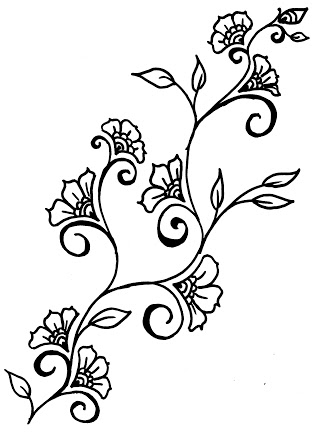
\includegraphics{figures/image1.png}
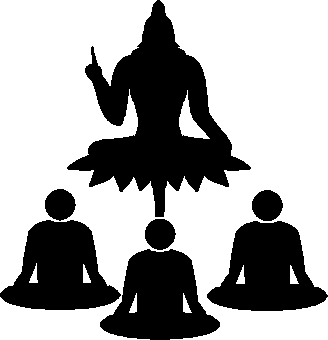
\includegraphics{figures/image2.png}
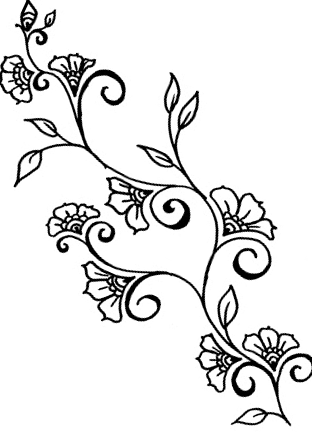
\includegraphics{figures/image1c.png}
\vskip 10pt
\setbox0=\vbox{\baselineskip=20pt
\lineskiplimit=0pt
\devanagarifont\Huge\bfseries #1
}
\newdimen\xdimen
\xdimen = \ht0
\advance\xdimen by28pt
\vbox to\xdimen{%
\vbox{\hbox to\textwidth{\rule{\textwidth}{1.6pt}}%
\kern -14pt
\hbox to\textwidth{\rule{\textwidth}{0.2pt}}
}
\vfill
\copy0
\vfill
\vbox{\hbox to\textwidth{\rule{\textwidth}{0.2pt}}%
\kern -13pt
\hbox to\textwidth{\rule{\textwidth}{1.6pt}}
}}
}}

\def\@part[#1]#2{%
    \ifnum \c@secnumdepth >-2\relax
      \refstepcounter{part}%
      \addcontentsline{toc}{part}{\eng{\thepart}\hspace{1em}#1}%
    \else
      \addcontentsline{toc}{part}{#1}%
    \fi
    \markboth{}{}%
    {\centering
     \interlinepenalty \@M
     \normalfont
     \ifnum \c@secnumdepth >-2\relax
       {\selectlanguage{english}\englishfont\huge\bfseries \partname\nobreakspace\thepart}
       \par
       \vskip 20\p@
     \fi
     \devanagarifont\Huge\bfseries #2\par}%
    \@endpart}

\makeatother

\selectlanguage{sanskrit}
\part{शास्त्रसम्बन्धीनि लेखनानि}

\lhead[\small\eng{\thepage}]{\small\dev{\leftmark}}

\input src/partII/01-chapter-24.tex
\input src/partII/02-chapter-27.tex
\input src/partII/03-chapter-15.tex
\input src/partII/04-chapter-16.tex
\input src/partII/05-chapter-10.tex
\input src/partII/06-chapter-34.tex
\input src/partII/07-chapter-11.tex
\input src/partII/08-chapter-32.tex
\input src/partII/09-chapter-20.tex
\input src/partII/10-chapter-13.tex
\selectlanguage{kannada}
\makeatletter
\renewcommand\chaptermark[1]{\markboth{\kannadafont #1}{}}
\def\@makechapterhead#1{{%
%~ \vspace*{50\p@}%
\centering
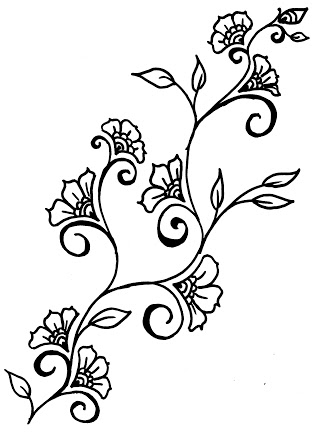
\includegraphics{figures/image1.png}
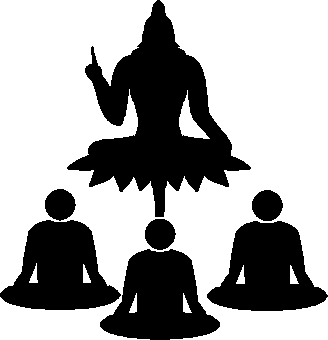
\includegraphics{figures/image2.png}
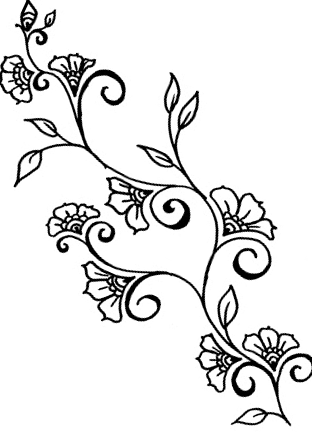
\includegraphics{figures/image1c.png}
\vskip 10pt
\setbox0=\vbox{\baselineskip=20pt
\lineskiplimit=0pt
\kannadafont\Huge\bfseries #1
}
\newdimen\xdimen
\xdimen = \ht0
\advance\xdimen by28pt
\vbox to\xdimen{%
\vbox{\hbox to\textwidth{\rule{\textwidth}{1.6pt}}%
\kern -12pt
\hbox to\textwidth{\rule{\textwidth}{0.2pt}}
}
\vfill
\copy0
\vfill
\vbox{\hbox to\textwidth{\rule{\textwidth}{0.2pt}}%
\kern -11pt
\hbox to\textwidth{\rule{\textwidth}{1.6pt}}
}}
}}
\makeatother
\input src/partII/11-chapter-41.tex
\selectlanguage{sanskrit}
\makeatletter
\renewcommand\chaptermark[1]{\markboth{#1}{}}
\def\@makechapterhead#1{{%
\vspace*{50\p@}%
\centering
\setbox0=\vbox{\baselineskip=20pt
\lineskiplimit=0pt
\devanagarifont\Huge\bfseries #1
}
\newdimen\xdimen
\xdimen = \ht0
\advance\xdimen by28pt
\vbox to\xdimen{%
\vbox{\hbox to\textwidth{\rule{\textwidth}{1.6pt}}%
\kern -14pt
\hbox to\textwidth{\rule{\textwidth}{0.2pt}}
}
\vfill
\copy0
\vfill
\vbox{\hbox to\textwidth{\rule{\textwidth}{0.2pt}}%
\kern -13pt
\hbox to\textwidth{\rule{\textwidth}{1.6pt}}
}}
}}
\makeatother
\input src/partII/12-chapter-83.tex
\input src/partII/13-chapter-21.tex
\input src/partII/14-chapter-22.tex
\input src/partII/15-chapter-25.tex
\input src/partII/16-chapter-28.tex
\input src/partII/17-chapter-85.tex
\input src/partII/18-chapter-38.tex
\input src/partII/19-chapter-29.tex
\input src/partII/20-chapter-30.tex
\input src/partII/21-chapter-86.tex
\input src/partII/22-chapter-37.tex
\input src/partII/23-chapter-18.tex
\input src/partII/24-chapter-26.tex
\input src/partII/25-chapter-12.tex
\input src/partII/26-chapter-31.tex
\selectlanguage{kannada}
\makeatletter
\renewcommand\chaptermark[1]{\markboth{\kannadafont #1}{}}
\def\@makechapterhead#1{{%
\vspace*{50\p@}%
\centering
\setbox0=\vbox{\baselineskip=20pt
\lineskiplimit=0pt
\kannadafont\Huge\bfseries #1
}
\newdimen\xdimen
\xdimen = \ht0
\advance\xdimen by28pt
\vbox to\xdimen{%
\vbox{\hbox to\textwidth{\rule{\textwidth}{1.6pt}}%
\kern -12pt
\hbox to\textwidth{\rule{\textwidth}{0.2pt}}
}
\vfill
\copy0
\vfill
\vbox{\hbox to\textwidth{\rule{\textwidth}{0.2pt}}%
\kern -11pt
\hbox to\textwidth{\rule{\textwidth}{1.6pt}}
}}
}}
\makeatother
\input src/partII/27-chapter-40.tex
\selectlanguage{sanskrit}
\makeatletter
\renewcommand\chaptermark[1]{\markboth{#1}{}}
\def\@makechapterhead#1{{%
\vspace*{50\p@}%
\centering
\setbox0=\vbox{\baselineskip=20pt
\lineskiplimit=0pt
\devanagarifont\Huge\bfseries #1
}
\newdimen\xdimen
\xdimen = \ht0
\advance\xdimen by28pt
\vbox to\xdimen{%
\vbox{\hbox to\textwidth{\rule{\textwidth}{1.6pt}}%
\kern -14pt
\hbox to\textwidth{\rule{\textwidth}{0.2pt}}
}
\vfill
\copy0
\vfill
\vbox{\hbox to\textwidth{\rule{\textwidth}{0.2pt}}%
\kern -13pt
\hbox to\textwidth{\rule{\textwidth}{1.6pt}}
}}
}}
\makeatother
\input src/partII/28-chapter-19.tex
\input src/partII/29-chapter-33.tex
\input src/partII/30-chapter-80.tex
\input src/partII/31-chapter-35.tex
\input src/partII/32-chapter-09.tex
\input src/partII/33-chapter-82.tex
\input src/partII/34-chapter-78.tex
\input src/partII/35-chapter-14.tex
\input src/partII/36-chapter-08.tex
\input src/partII/37-chapter-79.tex
\input src/partII/39-chapter-23.tex
\input src/partII/40-chapter-17.tex
\input src/partII/41-chapter-39.tex
\input src/partII/42-chapter-36.tex

	
\makeatletter

\def\@part[#1]#2{%
    \ifnum \c@secnumdepth >-2\relax
      \refstepcounter{part}%
      \addcontentsline{toc}{part}{\eng{\thepart}\hspace{1em}\kan{#1}}%
    \else
      \addcontentsline{toc}{part}{#1}%
    \fi
    \markboth{}{}%
    {\centering
     \interlinepenalty \@M
     \normalfont
     \ifnum \c@secnumdepth >-2\relax
       {\selectlanguage{english}\englishfont\huge\bfseries \partname\nobreakspace\thepart}
       \par
       \vskip 20\p@
     \fi
     \kannadafont\Huge\bfseries #2\par}%
    \@endpart}

\def\@makechapterhead#1{{%
\vspace*{50\p@}%
\centering
\setbox0=\vbox{\baselineskip=20pt
\lineskiplimit=0pt
\kannadafont\Huge\bfseries #1
}
\newdimen\xdimen
\xdimen = \ht0
\advance\xdimen by28pt
\vbox to\xdimen{%
\vbox{\hbox to\textwidth{\rule{\textwidth}{1.6pt}}%
\kern -12pt
\hbox to\textwidth{\rule{\textwidth}{0.2pt}}
}
\vfill
\copy0
\vfill
\vbox{\hbox to\textwidth{\rule{\textwidth}{0.2pt}}%
\kern -11pt
\hbox to\textwidth{\rule{\textwidth}{1.6pt}}
}}
}}

\renewcommand\section{\@startsection {section}{1}{\z@}%
                                   {-2.2ex \@plus -1.3ex \@minus -.3ex}%
                                   {1ex \@plus.2ex}%
                                   {\kannadafont\Large\bfseries}}
\renewcommand\chaptermark[1]{\markboth{\kannadafont #1}{}}                                   

\makeatother

\part{ಶ್ರೀಯುತ ಗಂಗಾಧರ ಭಟ್ಟರ ಒಡನಾಡಿಗಳ ಒಳನುಡಿ}

\selectlanguage{kannada}

\input src/partIII/01-chapter-42.tex
\selectlanguage{sanskrit}
\renewcommand\chaptermark[1]{\markboth{#1}{}}
\lhead[\small\thepage]{\small\dev{\leftmark}}

\makeatletter

\def\@makechapterhead#1{{%
\vspace*{50\p@}%
\centering
\setbox0=\vbox{\baselineskip=20pt
\lineskiplimit=0pt
\devanagarifont\Huge\bfseries #1
}
\newdimen\xdimen
\xdimen = \ht0
\advance\xdimen by28pt
\vbox to\xdimen{%
\vbox{\hbox to\textwidth{\rule{\textwidth}{1.6pt}}%
\kern -12pt
\hbox to\textwidth{\rule{\textwidth}{0.2pt}}
}
\vfill
\copy0
\vfill
\vbox{\hbox to\textwidth{\rule{\textwidth}{0.2pt}}%
\kern -11pt
\hbox to\textwidth{\rule{\textwidth}{1.6pt}}
}}
}}
\makeatother


\input src/partIII/02-chapter-04.tex
\input src/partIII/03-chapter-03.tex
\input src/partIII/04-chapter-05.tex
\input src/partIII/05-chapter-06.tex
\input src/partIII/06-chapter-07.tex
\clearpage

\selectlanguage{kannada}
\renewcommand\chaptermark[1]{\markboth{#1}{}}
\lhead[\small\thepage]{\small\kan{\leftmark}}
\makeatletter

\def\@makechapterhead#1{{%
\vspace*{50\p@}%
\centering
\setbox0=\vbox{\baselineskip=20pt
\lineskiplimit=0pt
\kannadafont\Huge\bfseries #1
}
\newdimen\xdimen
\xdimen = \ht0
\advance\xdimen by28pt
\vbox to\xdimen{%
\vbox{\hbox to\textwidth{\rule{\textwidth}{1.6pt}}%
\kern -12pt
\hbox to\textwidth{\rule{\textwidth}{0.2pt}}
}
\vfill
\copy0
\vfill
\vbox{\hbox to\textwidth{\rule{\textwidth}{0.2pt}}%
\kern -11pt
\hbox to\textwidth{\rule{\textwidth}{1.6pt}}
}}
}}
\makeatother
\input src/partIII/07-chapter-43.tex
\input src/partIII/08-chapter-44.tex
\input src/partIII/09-chapter-46.tex
\input src/partIII/10a-chapter-45.tex
\input src/partIII/11a-chapter-49.tex
\input src/partIII/11b-chapter-47.tex
\input src/partIII/11c-chapter-84.tex
\input src/partIII/12-chapter-64.tex
\input src/partIII/13-chapter-48.tex
\input src/partIII/14-chapter-51.tex
\input src/partIII/15-chapter-52.tex
\input src/partIII/16-chapter-54.tex
\input src/partIII/17-chapter-53.tex
\input src/partIII/18-chapter-61.tex
\input src/partIII/19-chapter-55.tex
\input src/partIII/20-chapter-50.tex
\input src/partIII/21-chapter-63.tex
\input src/partIII/22-chapter-58.tex
\input src/partIII/23-chapter-60.tex
\input src/partIII/24-chapter-69.tex
\input src/partIII/25-chapter-56.tex
\input src/partIII/26-chapter-62.tex
\input src/partIII/27-chapter-66.tex
\input src/partIII/28-chapter-90.tex
\input src/partIII/29-chapter-91.tex
\input src/partIII/30-chapter-57.tex
\input src/partIII/31-chapter-67.tex
\input src/partIII/32-chapter-81.tex
\input src/partIII/33-chapter-72.tex
\input src/partIII/34-chapter-71.tex
\input src/partIII/35a-chapter-70.tex
\input src/partIII/35b-chapter-65.tex
\input src/partIII/36-chapter-68.tex
\input src/partIII/37-chapter-59.tex
\input src/partIII/38-chapter-89.tex
\selectlanguage{sanskrit}
\makeatletter
\renewcommand\chaptermark[1]{\markboth{#1}{}}
\lhead[\small\thepage]{\small\dev{\leftmark}}
\def\@makechapterhead#1{{%
\vspace*{50\p@}%
\centering
\setbox0=\vbox{\baselineskip=20pt
\lineskiplimit=0pt
\devanagarifont\Huge\bfseries #1
}
\newdimen\xdimen
\xdimen = \ht0
\advance\xdimen by28pt
\vbox to\xdimen{%
\vbox{\hbox to\textwidth{\rule{\textwidth}{1.6pt}}%
\kern -12pt
\hbox to\textwidth{\rule{\textwidth}{0.2pt}}
}
\vfill
\copy0
\vfill
\vbox{\hbox to\textwidth{\rule{\textwidth}{0.2pt}}%
\kern -11pt
\hbox to\textwidth{\rule{\textwidth}{1.6pt}}
}}
}}
\makeatother
\input src/partIII/39-chapter-87.tex
\input src/partIII/40-chapter-77.tex
\clearpage
\selectlanguage{english}
\makeatletter

\def\@makechapterhead#1{{%
\vspace*{50\p@}%
\centering
\setbox0=\vbox{\baselineskip=20pt
\lineskiplimit=0pt
\englishfont\Huge\bfseries #1
}
\newdimen\xdimen
\xdimen = \ht0
\advance\xdimen by28pt
\vbox to\xdimen{%
\vbox{\hbox to\textwidth{\rule{\textwidth}{1.6pt}}%
\kern -12pt
\hbox to\textwidth{\rule{\textwidth}{0.2pt}}
}
\vfill
\copy0
\vfill
\vbox{\hbox to\textwidth{\rule{\textwidth}{0.2pt}}%
\kern -11pt
\hbox to\textwidth{\rule{\textwidth}{1.6pt}}
}}
}}
\makeatother
\lhead[\small\thepage]{\small\eng{\leftmark}}
\rhead[{\small\kan{ಜ್ಞಾನಗಂಗಾಧರ}}]{\small\thepage}
\chead[]{}
\cfoot[]{}
\input src/partIII/41-chapter-73.tex
\input src/partIII/42-chapter-74.tex
\input src/partIII/43-chapter-75.tex
\input src/partIII/44-chapter-76.tex

\end{document}

